%% USPSC-Cap3-MateriaisMetodos.tex

\chapter[Materiais e métodos]{Materiais e métodos}
\label{cap_metodos}

Nesta versão, este capítulo apresenta a caracterização da base de dados usada no trabalho. A Seção~\ref{sec_base} apresenta a base MBG-V2: sua origem, as condições em que os voos foram feitos, a estrutura dos arquivos, as estatísticas das anotações e da telemetria, as verificações de integridade e as limitações da base. As estatísticas desta seção foram calculadas pelo autor a partir dos 26 voos da base, com o tratamento e as exclusões descritos na Seção~\ref{sec_base_integridade}.
% As seções seguintes (detector, associação de focos por telemetria, estratégias de inferência e protocolo de medição de energia) serão acrescentadas aqui.

\section{Base de dados MBG-V2}
\label{sec_base}

\subsection{Origem e aquisição}
\label{sec_base_origem}

A base \textit{Mosquito Breeding Grounds V2} (MBG-V2) foi publicada pelo Laboratório de Sinais, Multimídia e Telecomunicações da COPPE/UFRJ \cite{smt2024mbgv2} e sucede a base MBG, do mesmo grupo \cite{passos2022mbg}. A MBG foi usada no desafio \textit{Automatic Detection of Mosquito Breeding Grounds}, promovido na conferência ICIP de 2023, que recebeu resultados de participantes do Brasil, do Catar e da Espanha \cite{passos2023icip}. O trabalho vencedor combinou um detector YOLOv7 com uma etapa de rastreamento para associar as detecções de um mesmo objeto ao longo do vídeo \cite{laranjeira2023yolov7}.

A MBG-V2 reúne 26 voos sobre 13 regiões urbanas do município do Rio de Janeiro, identificadas pelas letras A a M, com dois voos por região. A base é distribuída em 26 arquivos compactados, um por voo, que somam 211,6~GiB, e inclui um polígono que delimita cada região. A soma das áreas desses polígonos é de 1,37~km$^2$. Os voos pertencem a duas campanhas. A região A foi imageada em junho de 2019, data registrada no voo 02, já que o registro do voo 01 não traz data. As regiões B a M foram imageadas entre outubro de 2020 (região B) e março de 2021. A Figura~\ref{fig_regioes}a mostra a localização das regiões: as regiões B a M ficam na porção oeste do município, a no máximo 13,7~km umas das outras, e a região A fica a 42,5~km da mais próxima delas.
% Pendência: o sítio da base não indica uma licença de uso explícita. Confirmar com os autores que o uso acadêmico está liberado e registrar aqui.

\begin{figure}[htb]
  \centering
  \caption{Localização das 13 regiões da base MBG-V2 no município do Rio de Janeiro e faixas imageadas pelos dois voos da região M}
  \label{fig_regioes}
  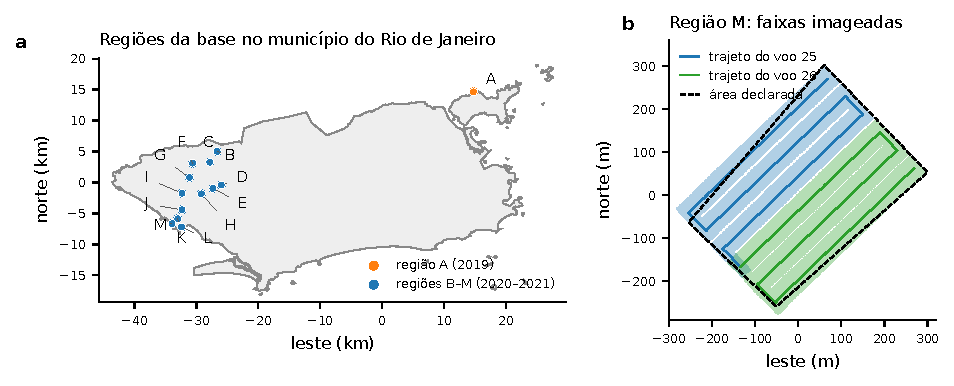
\includegraphics[width=\textwidth]{figuras/fig_mbgv2_regioes.pdf}
  \fonte{Elaborado pelo autor a partir dos polígonos e da telemetria da base MBG-V2 \cite{smt2024mbgv2} e da malha municipal do IBGE \cite{ibge2026malha}. (a) Cada ponto é o centro do polígono de uma região, em coordenadas locais norte-leste centradas no município. (b) As áreas coloridas são as faixas imageadas por cada voo, calculadas com o $GSD$ ajustado na Seção~\ref{sec_base_condicoes}; as linhas cheias são os trajetos da aeronave, e a linha tracejada é o polígono da região.}
\end{figure}

\subsection{Condições de voo e câmera}
\label{sec_base_condicoes}

Os vídeos e a telemetria informam a resolução das imagens, a taxa de quadros, a velocidade e a altitude registrada em cada voo. Para calcular a área de solo vista pela câmera, porém, é preciso conhecer também o $GSD$, isto é, quantos centímetros no solo correspondem a um pixel. Como a base não informa os parâmetros da câmera necessários à Equação~\eqref{eq_gsd}, essa escala foi estimada a partir das imagens e da telemetria. A seguir, são apresentados os dados registrados, o procedimento de estimativa e os valores obtidos.

\subsubsection{Dados registrados nos voos}

Em todos os voos, o \textit{gimbal} mantém a câmera apontada verticalmente para baixo, com ângulo de arfagem registrado de $-89{,}9^\circ$. A altitude da telemetria fica entre 39,8 e 40,1~m (percentis 5 e 95 de todas as amostras). Esse valor é medido em relação ao ponto de decolagem e não fornece, necessariamente, a altura da câmera sobre cada objeto imageado.

As principais diferenças entre as campanhas estão na velocidade e na configuração do vídeo. Na região A, o vídeo tem 4096 pixels de largura e 23,976 quadros por segundo, e a aeronave voa a cerca de 7,9~m/s. Nas regiões B a M, o vídeo tem 3840 pixels de largura e 29,97 quadros por segundo, e a velocidade fica perto de 4,1~m/s. A Tabela~\ref{tab_campanhas} separa essas informações dos valores de $GSD$, pegada e número de observações estimados neste trabalho.

\begin{table}[htb]
  \centering
  \caption{Condições de aquisição e grandezas estimadas nas duas campanhas da base MBG-V2}
  \label{tab_campanhas}
  \resizebox{\textwidth}{!}{%
  \begin{tabular}{lcc}
    \hline
    & Região A (voos 01 e 02) & Regiões B a M (voos 03 a 26) \\
    \hline
    \multicolumn{3}{l}{\textit{Informações dos vídeos e da telemetria}} \\
    Período & jun. 2019 & out. 2020 a mar. 2021 \\
    Resolução do vídeo (pixels) & $4096 \times 2160$ & $3840 \times 2160$ \\
    Taxa de quadros, $f_q$ (quadros/s) & 23,976 & 29,97 \\
    Codificação do vídeo & MJPG & MJPG (19 voos) ou H.264 (5 voos) \\
    Velocidade mediana, $V$ (m/s) & 7,88--7,93 & 4,06--4,16 \\
    Altitude relativa à decolagem (m) & 40 & 40 \\
    Registro de telemetria & uma linha por quadro & cerca de 10 ou 20 linhas/s \\
    \hline
    \multicolumn{3}{l}{\textit{Grandezas estimadas neste trabalho}} \\
    $GSD$ ajustado (cm/pixel) & 1,21--1,23 & 1,20--1,78 \\
    Largura da pegada, $w$ (m) & 49,6--50,4 & 46,1--68,4 \\
    Comprimento da pegada, $L$ (m) & 26,1--26,6 & 25,9--38,4 \\
    Quadros por ponto do solo, $n_v$ & 79--81 & 190--283 \\
    \hline
  \end{tabular}}
  \fonte{Elaborado pelo autor a partir dos vídeos, das anotações e da telemetria da base MBG-V2 \cite{smt2024mbgv2}. Os intervalos indicam o menor e o maior valor entre os voos da campanha. O $GSD$ foi ajustado pelo procedimento descrito nesta seção; $w$, $L$ e $n_v$ foram calculados pelas Equações~\eqref{eq_pegada} e \eqref{eq_visibilidade}.}
\end{table}

\subsubsection{Princípio da estimativa do GSD}

O ajuste explora os objetos anotados que permanecem parados no solo. À medida que a aeronave avança, um mesmo objeto aparece em posições diferentes da imagem, mas sua posição no terreno deve permanecer a mesma. Uma \textit{trilha} reúne as caixas anotadas que acompanham esse objeto ao longo dos quadros. Ao projetar essas caixas no solo pela Equação~\eqref{eq_georref}, obtém-se uma sequência de posições: quanto mais próximas elas ficarem, maior será a consistência da projeção daquela trilha.

O $GSD$ controla a escala dessa projeção. Se ele for pequeno demais, a distância calculada entre a aeronave e o objeto será subestimada, e a posição projetada acompanhará parte do movimento da aeronave. Se for grande demais, a distância será superestimada, e a posição projetada se deslocará no sentido oposto. O procedimento procura, portanto, o valor de $GSD$ que deixa as posições de cada objeto mais concentradas ao longo do voo. Não é necessário conhecer previamente a posição verdadeira do objeto para medir essa concentração. A Figura~\ref{fig_estimativa_gsd} ilustra o princípio.

\begin{figure}[htbp]
  \centering
  \caption{Efeito do $GSD$ adotado na projeção de um objeto parado}
  \label{fig_estimativa_gsd}
  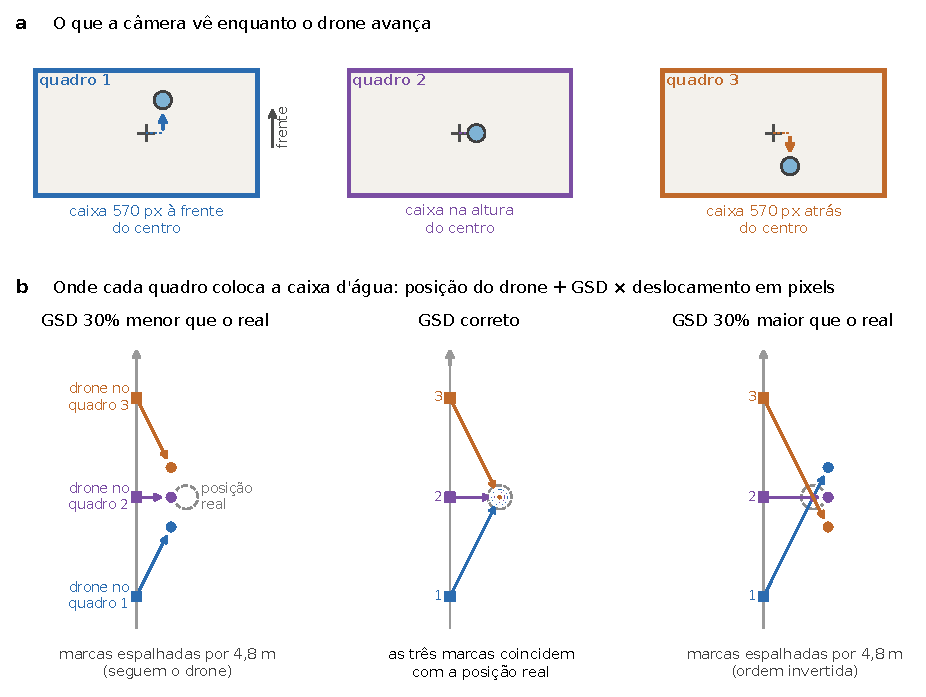
\includegraphics[width=0.9\textwidth]{figuras/fig_estimativa_gsd.pdf}
  \fonte{Elaborado pelo autor, com valores ilustrativos. (a) O mesmo objeto aparece em três posições da imagem à medida que a aeronave avança. (b) Cada caixa é projetada no solo pela Equação~\eqref{eq_georref}. No modelo ideal, o $GSD$ correto faz as projeções coincidirem; um valor 30\% menor ou maior produz dispersão, em sentidos opostos. O círculo tracejado indica a posição real do objeto.}
\end{figure}

Essa relação pode ser escrita a partir de duas posições no plano horizontal: a do objeto, $\mathbf{x}_{\mathrm{obj}}$, e a da aeronave em cada quadro, $\mathbf{x}_{\mathrm{aer}}$. Seja $GSD_{\mathrm{real}}$ a escala verdadeira, desconhecida. No modelo de projeção com visada vertical da Seção~\ref{sec_georref}, após considerar a rotação pela guinada, a projeção calculada com um valor candidato de $GSD$ é
\begin{equation*}
  \mathbf{x}_{\mathrm{proj}} = \mathbf{x}_{\mathrm{aer}} + \frac{GSD}{GSD_{\mathrm{real}}}\,\bigl(\mathbf{x}_{\mathrm{obj}} - \mathbf{x}_{\mathrm{aer}}\bigr).
\end{equation*}
Subtraindo a posição verdadeira do objeto, obtém-se
\begin{equation*}
  \mathbf{x}_{\mathrm{proj}} - \mathbf{x}_{\mathrm{obj}} = \left(1 - \frac{GSD}{GSD_{\mathrm{real}}}\right)\bigl(\mathbf{x}_{\mathrm{aer}} - \mathbf{x}_{\mathrm{obj}}\bigr).
\end{equation*}
Quando $GSD=GSD_{\mathrm{real}}$, o fator entre parênteses é zero e as projeções coincidem com a posição do objeto. Nos demais casos, a expressão mostra quanto do movimento da aeronave aparece como deslocamento indevido do objeto. Para uma trilha que atravessa todo o campo de visão em voo retilíneo, com orientação constante, a aeronave percorre aproximadamente o comprimento $L$ da pegada. As projeções se espalham então por um segmento de comprimento $\lvert1-GSD/GSD_{\mathrm{real}}\rvert L$. Como exemplo desse modelo ideal, um erro de 10\% na escala produziria cerca de 3 a 4~m de espalhamento para os comprimentos de pegada da Tabela~\ref{tab_campanhas}; esse espalhamento não é uma medição dos voos.

\subsubsection{Procedimento de ajuste}

O ajuste foi feito separadamente para cada voo. As caixas foram amostradas a cada 5 quadros, e foram usadas apenas trilhas com pelo menos 5 amostras. Para cada valor candidato de $GSD$, aplicou-se a seguinte sequência:
\begin{enumerate}
  \item projetar no solo cada caixa $k$ de cada trilha $j$, obtendo a posição $\mathbf{x}_{jk}(GSD)$ em coordenadas norte-leste;
  \item calcular o centro da trilha, $\tilde{\mathbf{x}}_j(GSD)$, pela mediana de cada coordenada das posições projetadas;
  \item calcular a dispersão da trilha como a mediana das distâncias de suas projeções a esse centro;
  \item calcular a dispersão do voo como a mediana das dispersões de todas as trilhas usadas no ajuste.
\end{enumerate}
Escolheu-se o $GSD$ que minimiza essa última medida. A busca percorreu valores de 0,80 a 2,20~cm/pixel, inicialmente com passo de 0,05~cm/pixel e depois com refinamento de 0,01~cm/pixel. A Equação~\eqref{eq_gsd_ajuste} reúne os quatro passos e a escolha do mínimo:
\begin{equation}
  \widehat{GSD} \in \arg\min_{GSD\in\mathcal{S}}\
  \underbrace{\operatorname*{med}_{j}\Biggl[\ \underbrace{\operatorname*{med}_{k}\ \bigl\lVert \mathbf{x}_{jk}(GSD) - \tilde{\mathbf{x}}_j(GSD) \bigr\rVert}_{\text{dispersão da trilha } j}\ \Biggr]}_{\text{dispersão do voo}},
  \label{eq_gsd_ajuste}
\end{equation}
em que $\mathcal{S}$ é o conjunto de valores positivos pesquisados. A mediana interna resume as distâncias dentro de uma trilha; a externa resume as trilhas do voo. O operador $\arg\min$ identifica os valores de $GSD$ que produzem a menor dispersão, e $\widehat{GSD}$ é um deles. Usar medianas reduz a influência de caixas mal posicionadas ou de objetos que se movem, como sacos plásticos levados pelo vento.\footnote{O centro de cada trilha é calculado por medianas coordenada a coordenada no referencial norte-leste, procedimento que não é, em geral, invariante a uma rotação dos eixos. Eventuais empates na busca do mínimo exigem uma regra de escolha registrada na implementação.}

\subsubsection{Valores obtidos e interpretação}

O $GSD$ ajustado varia de 1,20 a 1,78~cm/pixel entre os voos, com mediana de 1,42~cm/pixel e intervalo interquartil de 1,33 a 1,50~cm/pixel. A mediana é próxima do valor ilustrativo de 1,4~cm/pixel usado na Figura~\ref{fig_geometria}. Com o ajuste, a dispersão mediana das trilhas fica entre 0,24 e 0,85~m, conforme o voo. Essa dispersão mede a consistência das posições de um mesmo objeto ao longo do vídeo; ela não mede, por si só, o erro em relação à sua posição geográfica verdadeira.

Como comparação, ao usar $GSD=0$, a projeção coincide com a posição da aeronave em todos os quadros. A dispersão mediana das trilhas passa então para 6,2 a 9,1~m. Esses valores são da ordem de $L/4$, entre 6,5 e 9,6~m para as pegadas da Tabela~\ref{tab_campanhas}: em uma travessia completa e uniformemente amostrada de um segmento de comprimento $L$, a distância mediana ao centro é $L/4$. O caso $GSD=0$ serve apenas como referência para essa comparação e não integra o conjunto de escalas positivas pesquisadas no ajuste.

Embora a altitude registrada seja próxima de 40~m em todos os voos, isso não implica a mesma distância entre câmera e terreno. Diferenças de cota entre o ponto de decolagem e a área imageada são uma explicação possível para parte da variação do $GSD$. Essa hipótese não foi verificada, e a base não informa o modelo da aeronave nem os parâmetros da câmera para uma conferência independente da escala.

Com o $GSD$ ajustado, foram calculados a largura e o comprimento da pegada e o número de quadros por ponto do solo apresentados na Tabela~\ref{tab_campanhas}. Pela Equação~\eqref{eq_visibilidade}, o tempo de permanência de um ponto no campo de visão, $t_v=L/V$, é de 3,3--3,4~s na região A e de 6,4--9,4~s nas demais. As durações medianas das trilhas anotadas, de 3,4~s e 7,2~s, respectivamente, são compatíveis com esses intervalos.

No regime observado, com $V/f_q<L$, a fração nova de cada quadro é $V/(f_qL)$: de 1,24 a 1,27\% na região A e de 0,35 a 0,53\% nas regiões B a M. Assim, um ponto do solo aparece em cerca de 80 quadros na região A e em 190 a 280 nas demais. A maior velocidade e a menor taxa de quadros da primeira campanha reduzem, portanto, a redundância disponível para a memória geográfica.

\subsection{Estrutura dos dados}
\label{sec_base_estrutura}

Cada voo da base é composto por quatro elementos, gravados sobre o mesmo relógio:
\begin{itemize}
  \item o vídeo, em arquivo AVI, codificado em MJPG (21 voos, de 3,6--11,2~GiB cada) ou em H.264 (voos 17 e 23 a 26, de 1,1--1,9~GiB cada);
  \item as anotações, em um arquivo XML no formato da ferramenta CVAT, em modo de interpolação: cada objeto é uma trilha, com identificador e classe, que contém uma caixa delimitadora em cada quadro em que o objeto está visível, além de atributos que indicam os quadros-chave, a oclusão e a saída do objeto do campo de visão;
  \item o registro de telemetria do controlador de voo, em arquivo CSV com 92 colunas (93 na região A, que tem uma coluna adicional com o tempo do vídeo), que inclui posição, velocidades, atitude, ângulos do \textit{gimbal} e os dados da bateria: tensão, corrente, carga restante, porcentagem restante e tensão de cada célula;
  \item quadros do vídeo em PNG, a uma taxa de um quadro por segundo (um a cada 24 quadros na região A e um a cada 30 nas demais).
\end{itemize}

Neste trabalho, chama-se \textit{trilha} o conjunto de caixas com o mesmo identificador, que corresponde a um objeto físico acompanhado enquanto permanece no campo de visão. Cada trilha reúne, em mediana, 210 caixas, uma por quadro. Dois cuidados são necessários na leitura das anotações. Primeiro, o campo \texttt{size} dos metadados do arquivo XML não é o número de objetos, mas a duração do vídeo em segundos; o número de objetos deve ser contado pelos identificadores de trilha distintos. Segundo, o número de quadros do vídeo é dado por \texttt{stop\_frame} + 1.

A sincronização entre o vídeo e a telemetria foi verificada com o mesmo critério da Equação~\eqref{eq_gsd_ajuste}: o registro de telemetria foi deslocado em relação ao vídeo, em passos de 0,1~s entre $-1$ e $+1$~s, e mediu-se a dispersão resultante. Em 20 dos 26 voos, o deslocamento que minimiza a dispersão está entre $-0{,}2$ e $+0{,}2$~s, e nos demais o ganho obtido com o deslocamento é de no máximo 3,5\%. Por isso, o vídeo e a telemetria são tratados como sincronizados, sem correção de defasagem.

\subsection{Estatísticas das anotações}
\label{sec_base_anotacoes}

A base soma 193.901 quadros, ou 1,83~h de vídeo, com 1.649.228 caixas delimitadoras agrupadas em 8.441 trilhas de 12 classes. A Tabela~\ref{tab_classes} resume as classes, a Figura~\ref{fig_exemplos_classes} mostra exemplos de cada uma, e a Figura~\ref{fig_anotacoes} mostra como os objetos se distribuem entre os voos.

\begin{table}[htb]
  \centering
  \caption{Classes da base MBG-V2: número de trilhas, presença nos voos e nas regiões e tamanho dos objetos}
  \label{tab_classes}
  \resizebox{\textwidth}{!}{%
  \begin{tabular}{lrrrrrrr}
    \hline
    Classe (rótulo na base) & Trilhas & \% & Voos & Regiões & Lado (pixels) & Lado (cm) & $<$ 32 pixels (\%) \\
    \hline
    caixa d'água (\texttt{watertank}) & 4.283 & 50,7 & 26 & 13 & 114 & 157 (135--173) & 0 \\
    vaso de planta (\texttt{potted\_plant}) & 1.203 & 14,3 & 26 & 13 & 40 & 56 (41--80) & 32 \\
    bueiro (\texttt{storm\_drain}) & 948 & 11,2 & 26 & 13 & 43 & 61 (53--70) & 6 \\
    piscina (\texttt{pool}) & 763 & 9,0 & 26 & 13 & 189 & 268 (206--362) & 1 \\
    pneu (\texttt{tire}) & 509 & 6,0 & 26 & 13 & 40 & 58 (52--64) & 13 \\
    balde (\texttt{bucket}) & 455 & 5,4 & 25 & 13 & 27 & 38 (33--50) & 67 \\
    saco plástico (\texttt{plastic\_bag}) & 90 & 1,1 & 21 & 13 & 49 & 70 (59--86) & 6 \\
    garrafa (\texttt{bottle}) & 69 & 0,8 & 8 & 7 & 17 & 26 (22--33) & 93 \\
    lixeira pequena (\texttt{small\_trash\_bin}) & 40 & 0,5 & 11 & 8 & 42 & 60 (46--68) & 12 \\
    poça (\texttt{puddle}) & 39 & 0,5 & 8 & 6 & 181 & 232 (175--372) & 0 \\
    lixeira grande (\texttt{large\_trash\_bin}) & 36 & 0,4 & 14 & 10 & 50 & 68 (62--82) & 6 \\
    caçamba (\texttt{dumpster}) & 6 & 0,1 & 4 & 4 & 388 & 626 (513--676) & 0 \\
    \hline
  \end{tabular}}
  \fonte{Elaborado pelo autor a partir das anotações da base MBG-V2 \cite{smt2024mbgv2}. O lado de cada trilha é a mediana de $\sqrt{\text{largura} \times \text{altura}}$ de suas caixas; em centímetros, é convertido com o $GSD$ ajustado do voo. As colunas de lado mostram a mediana entre as trilhas e, entre parênteses, os percentis 25 e 75.}
\end{table}

\begin{figure}[htb]
  \centering
  \caption{Exemplos das 12 classes da base MBG-V2}
  \label{fig_exemplos_classes}
  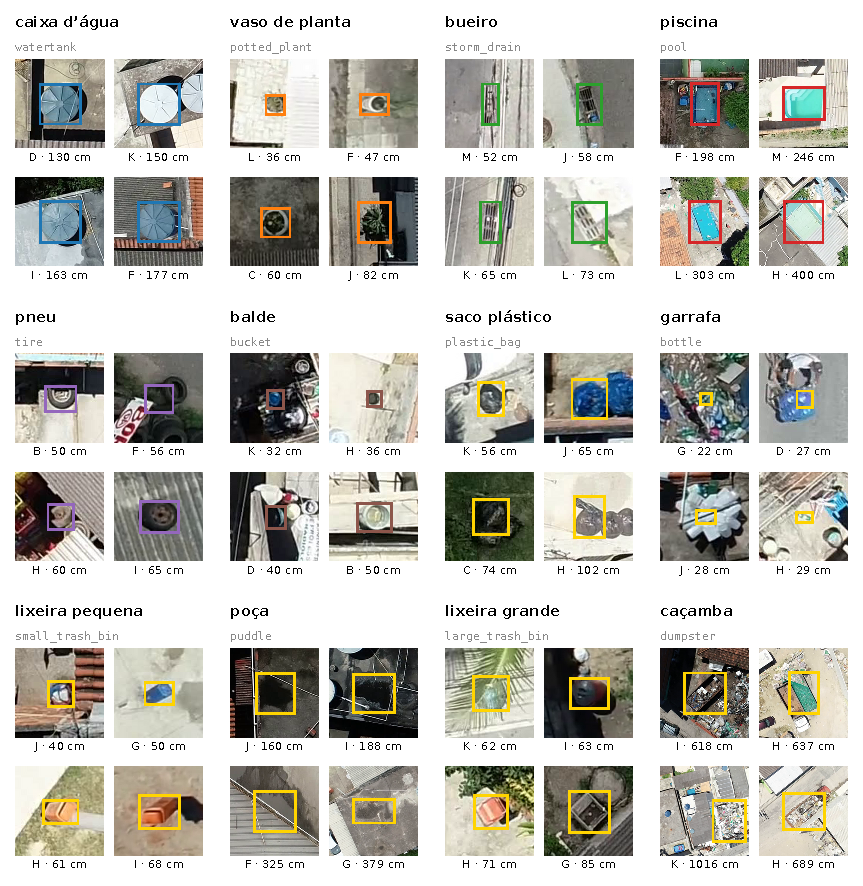
\includegraphics[width=\textwidth]{figuras/fig_mbgv2_exemplos_classes.pdf}
  \fonte{Elaborado pelo autor a partir dos quadros e das anotações da base MBG-V2 \cite{smt2024mbgv2}. Para cada classe, foram escolhidos quatro objetos de regiões diferentes, com tamanhos próximos dos percentis 20, 40, 60 e 80 da classe. Cada recorte é centrado na caixa anotada e tem lado igual a cerca de 2,2 vezes o maior lado da caixa, de modo que os recortes não estão na mesma escala. Abaixo de cada recorte, a região e o lado do objeto no solo.}
\end{figure}

A distribuição é desequilibrada. A classe caixa d'água responde por metade das trilhas, e as seis classes mais frequentes somam 96,7\% delas e aparecem em pelo menos 25 dos 26 voos e em todas as 13 regiões. As outras seis classes somam apenas 280 trilhas (3,3\%); garrafa e poça, por exemplo, aparecem em apenas 8 voos. Para essas classes, não há exemplos suficientes para uma avaliação separada por região.

O tamanho dos objetos no solo é coerente com o que cada classe representa: os pneus têm lado mediano de 58~cm, os baldes de 38~cm e as caixas d'água de 157~cm. Os objetos de menos de 32 pixels de lado são 10,7\% das trilhas, mas concentram-se em poucas classes: 93\% das garrafas, 67\% dos baldes e 32\% dos vasos de planta. Com o $GSD$ mediano, 32 pixels correspondem a cerca de 45~cm no solo. Pela Equação~\eqref{eq_spx}, o aumento da altitude reduz ainda mais o tamanho desses objetos em pixels, o que pode limitar a altura máxima da Equação~\eqref{eq_hmax}. O valor de 32 pixels é uma referência descritiva de tamanho; o limite de detecção depende da classe e do detector e deverá ser medido.

\begin{figure}[htb]
  \centering
  \caption{Densidade, composição e tamanho dos objetos anotados na base MBG-V2}
  \label{fig_anotacoes}
  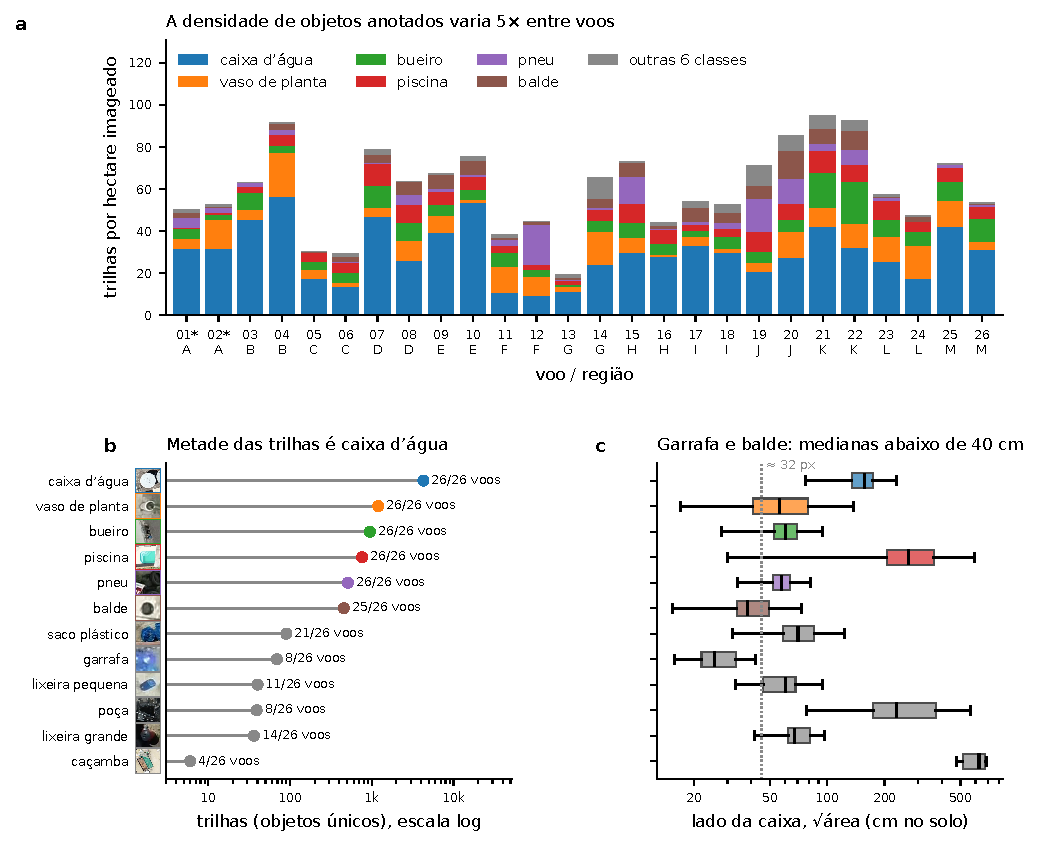
\includegraphics[width=\textwidth]{figuras/fig_mbgv2_anotacoes.pdf}
  \fonte{Elaborado pelo autor a partir das anotações e da telemetria da base MBG-V2 \cite{smt2024mbgv2}. (a) Trilhas por hectare de área imageada em cada voo; os voos marcados com asterisco são da campanha de 2019. (b) Número de trilhas por classe e número de voos em que a classe aparece; as miniaturas são exemplos reais de cada classe. (c) Lado dos objetos no solo; as caixas indicam os percentis 25 e 75, e as hastes se estendem até 1,5 vez o intervalo interquartil. A linha pontilhada corresponde a 32 pixels com o $GSD$ mediano de 1,42~cm/pixel.}
\end{figure}

Para comparar voos de durações diferentes, a densidade de objetos foi calculada como o número de trilhas por hectare de área imageada. A área imageada de cada voo, de 2,8--11,6~ha, é a união das pegadas da câmera ao longo do voo, calculada numa grade de 1~m com o $GSD$ ajustado e a guinada da câmera em cada instante. Somadas por região, essas áreas totalizam 1,42~km$^2$, e a razão entre a área imageada e a área do polígono de cada região fica entre 0,88--1,20, o que é coerente com o $GSD$ ajustado. A densidade varia de 19,4--94,8 trilhas por hectare entre os voos, com mediana de 60,1; o voo menos denso é o 13 e o mais denso é o 21. Em todos os voos há objetos na maior parte do vídeo: a fração de quadros com pelo menos um objeto tem mediana de 98,6\% e mínimo de 66,4\%.

A mesma grade permite verificar se um objeto pode ser contado duas vezes. Dentro de um voo, as passadas vizinhas quase não se sobrepõem: a área imageada é, em mediana, apenas 4\% menor que o produto da distância percorrida pela largura da pegada, com máximo de 27\% no voo 14. Os dois voos de cada região cobrem metades complementares, com sobreposição de 0,7--10,7\% da área imageada (Figura~\ref{fig_regioes}b). A baixa sobreposição sugere que o número de trilhas aproxima o número de objetos distintos, mas não permite quantificar quantos objetos foram anotados mais de uma vez. A possível duplicação deve ser considerada na definição e na interpretação da avaliação de focos únicos.

\subsection{Telemetria e energia dos voos}
\label{sec_base_energia}

A potência elétrica fornecida pela bateria foi calculada em cada amostra da telemetria como o produto da tensão pela corrente, $P_{el} = U\,I$, com a convenção de descarga positiva. A energia de cada voo foi obtida pela regra dos trapézios aplicada ao balanço da Equação~\eqref{eq_energia}, isto é, $E\approx\sum_i(P_{el,i}+P_{el,i+1})(t_{i+1}-t_i)/2$. A integração numérica é uma escolha deste trabalho, com os instantes e as lacunas tratados conforme a Seção~\ref{sec_base_integridade}. A energia por área foi então calculada como
\begin{equation}
  e_{\mathrm{voo}} = \frac{E}{A_{\mathrm{img}}},
  \label{eq_e_voo}
\end{equation}
em que $A_{\mathrm{img}}$ é a área imageada definida na Seção~\ref{sec_base_anotacoes}. Com $E$ em joules e $A_{\mathrm{img}}$ em m$^2$, o resultado em J/m$^2$ foi convertido para Wh/km$^2$ pelo fator $10^6/3600$. A Equação~\eqref{eq_e_voo} é a versão medida da Equação~\eqref{eq_e_area}: em vez de supor faixas sem sobreposição, ela usa a união das áreas imageadas, contabilizando uma única vez as regiões sobrepostas, inclusive nas curvas.

Nas regiões B a M, a potência mediana de cada voo varia de 173--190~W, com mediana de 182~W. A energia por voo vai de 25,6--68,0~kJ, e cada voo consome de 9--24 pontos percentuais da carga da bateria. Os 26 voos somam 330~Wh para percorrer 28,9~km. A energia por área nas regiões B a M tem mediana de 239~Wh/km$^2$, com variação de 204--271~Wh/km$^2$ entre os voos.

Os dois voos da região A, feitos a cerca de 7,9~m/s, consomem potência ligeiramente menor, de 170 e 172~W, e energia por área de 157 e 137~Wh/km$^2$, cerca de 39\% abaixo da mediana das demais regiões. Esse resultado é compatível com a curva de potência da Figura~\ref{fig_curva_potencia}, em que a potência diminui entre o pairado e a velocidade de mínima potência: dobrar a velocidade quase não altera a potência e, pela Equação~\eqref{eq_e_area}, reduz a energia por área. A comparação, porém, deve ser lida com cautela. Os voos da região A são de outra campanha, com outra configuração de vídeo, e não é possível confirmar que foram feitos com a mesma aeronave: os campos de número de série vêm vazios em todos os registros, e o único indício disponível é que todos os voos usam baterias de quatro células, cujo contador de ciclos passa de 11 em 2019 para 17 a 21 em 2020 e 2021.

Nas regiões B a M, todos os voos ocupam praticamente um único ponto de operação, a 40~m e cerca de 4,1~m/s. Por isso, a telemetria permite ancorar o modelo de potência da Seção~\ref{sec_voo_frente} nesse ponto, mas não calibrar a curva $P_{el}(V)$ inteira.

\subsection{Verificação de integridade e tratamento dos dados}
\label{sec_base_integridade}

Antes do uso, os 26 voos foram verificados quanto aos seguintes pontos:
\begin{itemize}
  \item o número de quadros declarado no cabeçalho de cada vídeo é igual ao número de quadros do arquivo de anotações, e o último quadro de cada vídeo é decodificado sem erro;
  \item os quadros em PNG são idênticos, pixel a pixel, aos quadros correspondentes do vídeo;
  \item a duração do registro de telemetria difere da duração do vídeo em no máximo 0,8~s, com exceção do voo 22, discutida abaixo;
  \item as trilhas apresentam baixa dispersão quando projetadas no solo (Seção~\ref{sec_base_condicoes}), o que indica consistência espacial dentro de cada trilha, mas não descarta a divisão de um mesmo objeto entre identificadores diferentes;
  \item a área imageada calculada a partir da telemetria é compatível com o polígono de cada região (Seção~\ref{sec_base_anotacoes}).
\end{itemize}

Foram encontrados três problemas, tratados como segue.
\begin{itemize}
  \item Em 5 voos (06, 07, 08, 14 e 22), o registro de telemetria tem interrupções breves, de cerca de 3~s, seguidas de algumas linhas em que os campos da bateria valem zero. Essas 99 linhas foram descartadas, e os valores nesses intervalos foram interpolados a partir das amostras vizinhas. Além disso, em 10 voos há linhas com carimbo de tempo repetido, a maioria nos voos 23 e 24, cujo registro é gravado em rajadas; dessas 713 linhas, manteve-se apenas a primeira de cada instante. As duas correções somam 812 linhas, 0,8\% do total.
  \item Nos voos 14 e 22, essas linhas aparecem no fim do registro e, no voo 14, estendem-se por 44~s além do fim do vídeo. No voo 22, a telemetria válida termina 9,8~s antes do fim do vídeo; esses quadros finais são excluídos das análises que dependem do georreferenciamento.
  \item A região A difere das demais em velocidade, taxa de quadros, resolução e data (Tabela~\ref{tab_campanhas}). Por isso, ela é tratada como um conjunto à parte: não será misturada às demais regiões no treino do detector e servirá para uma comparação exploratória em maior velocidade, sem isolar o efeito da velocidade das demais diferenças entre campanhas.
\end{itemize}
As seis classes com menos de 100 trilhas são mantidas nas estatísticas da base, mas não serão avaliadas separadamente por região.

\subsection{Representatividade e limitações}
\label{sec_base_limitacoes}

A base tem limitações que restringem a generalização dos resultados. Todos os voos foram feitos em uma única cidade, a uma única altitude nominal de 40~m e as anotações foram produzidas por um único grupo. O modelo da aeronave e os parâmetros da câmera não são informados, o que impede confirmar a uniformidade dos equipamentos entre as campanhas. A distribuição das classes é muito desequilibrada, com metade das trilhas em uma só classe e seis classes com poucos exemplos. Além disso, as 13 regiões cobrem, juntas, apenas 1,42~km$^2$, e as duas campanhas diferem em vários parâmetros ao mesmo tempo, o que impede separar o efeito de cada um.

Essas limitações orientam o protocolo do trabalho. Como a diversidade entre regiões é pequena, prevê-se uma avaliação que deixe uma região de fora a cada rodada, para medir a variação de desempenho em uma região não vista no treino. Como a altitude nominal é única, a redução da resolução das imagens será usada para emular a diminuição do tamanho dos objetos em pixels associada ao aumento da altura (Equação~\eqref{eq_spx}). Essa operação não reproduz todas as mudanças de perspectiva, oclusão e área coberta de um voo em outra altitude. Os voos a 10 e 25~m da base MBG \cite{passos2022mbg} servirão como referência complementar, sob outras condições de aquisição, sem validar diretamente a extrapolação para altitudes acima de 40~m.
